\chapter{Ongelmat JavaScriptin staattisessa tyypittämisessä}

\section{Luotettavuus, täydellisyys ja käytännöllisyys}

\begin{figure}
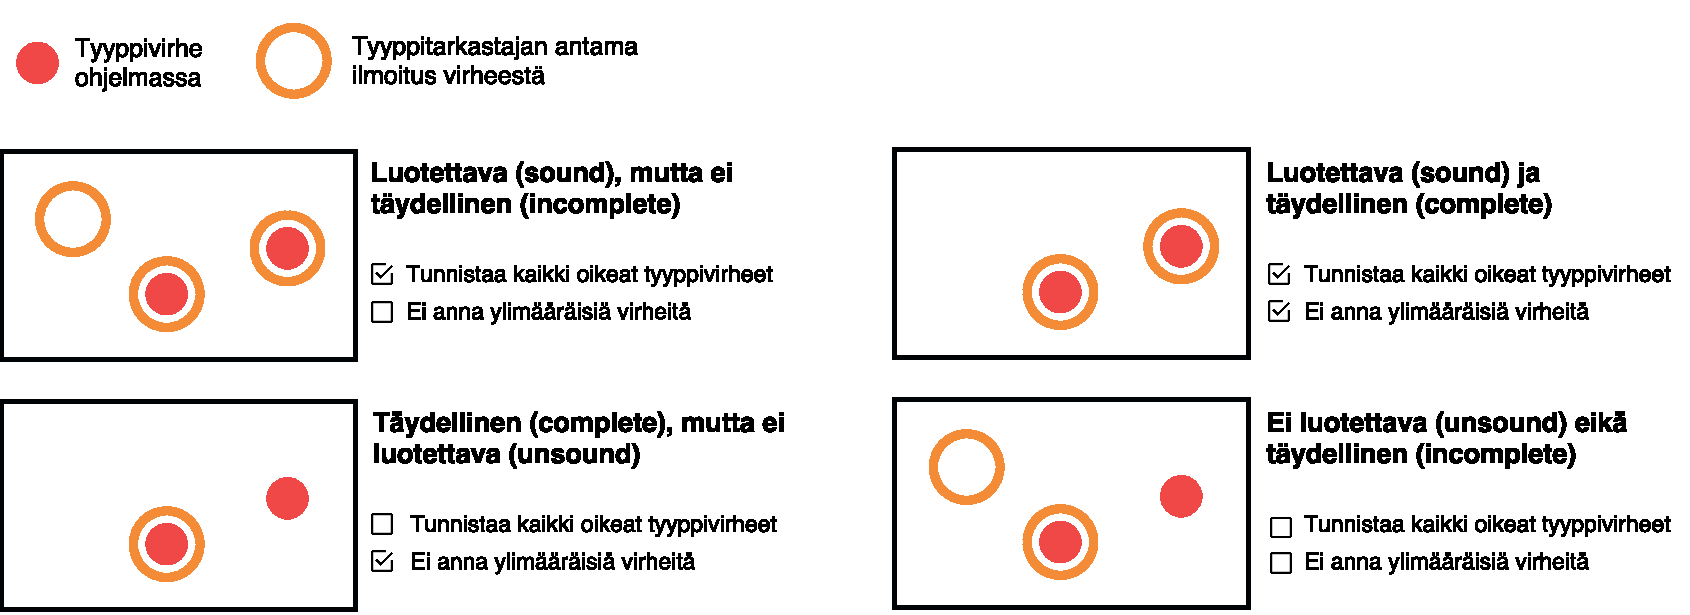
\includegraphics[width=\textwidth]{images/soundness_completeness2.pdf}
\caption{Tyyppijärjestelmän luotettavuus ja täydellisyys}
\end{figure}

Tyyppijärjestelmän luotettavuus (soundness) kuvaa sitä, kuinka suuren osan
mahdollisista ohjelmointivirheistä se estää. Täysin luotettava (sound)
tyyppijärjestelmä estää kaikki sellaiset virheet jotka sen on tarkoitus
estää \cite{CSE_ProgrammingLanguages}. Täydellisyys (completeness)
puolestaan kertoo salliiko tyyppijärjestelmä kielen sellaiset ominaisuudet
jotka eivät olisi ajonaikana tyyppivirheitä \cite{TypesAndProgrammingLanguages, CSE_ProgrammingLanguages}.

Jotta JavaScriptiä analysoiva tyyppijärjestelmä olisi luotettava, sen on
annettava virhe esimerkiksi seuraavasta ohjelmasta:

\begin{minipage}{\linewidth}
\begin{lstlisting}[caption={Virheellinen JavaScript-ohjelma: Lisätyllä tuotteella ei ole nimeä.}]
function osta(ostos) {
  lisaaTuote({
    nimi: ostos.nimi,
    hinta: ostos.hinta
  });
}

osta({ nimi: 'juusto', hinta: 5 });
osta({ hinta: 5 });
\end{lstlisting}
\label{fig:soundness_test}
\end{minipage}

Toisaalta jotta JavaScriptiä analysoiva tyyppijärjestelmä olisi täydellinen,
sen on sallittava tämä korjattu versio ylläolevasta ohjelmasta:

\begin{minipage}{\linewidth}
\begin{lstlisting}[caption={Toimiva JavaScript-ohjelma: Virheelliseltä kutsulta on suojauduttu tarkistuksella.}]
function osta(ostos) {
  if (typeof ostos.nimi === 'string') {
    lisaaTuote({
      nimi: ostos.nimi,
      hinta: ostos.hinta
    });
  }
}

osta({ nimi: 'juusto', hinta: 5 });
osta({ hinta: 5 });
\end{lstlisting}
\label{fig:completeness_test}
\end{minipage}

Esimerkit \ref{fig:soundness_test} ja \ref{fig:completeness_test} toimivat
odotetulla tavalla Flow:ssa. TypeScript vaatii eksplisiittisen tyyppiannotaation
osta-funktiolle, mutta toimii muuten samalla tavalla.

